% Provenance (never printed): see sources/outline_sources.md (Year 3:
% planetary atmospheres, escape, the runaway greenhouse, Mars, Titan,
% habitability).
% Brief: sources/book5/BRIEFS.md, ch. 27. Curves from figdata/bachelor-3/
% jeans_escape.py (escape parameter and escaping fraction at the exobases
% of Venus, the Earth, Mars and Titan), runaway_greenhouse.py (an
% illustrative grey model of a moist atmosphere: OLR against surface
% temperature) and habitability.py (the habitable-zone fits of Kopparapu et
% al. 2013; the phase boundaries of water and methane with the surface
% states of four bodies). Exercise and problem values in the Book 5 scratch
% calculator calc/ch27.py. Kepos and its star are invented.
\chapter{الغلاف الجوي للكواكب وصلاحيتها للحياة}\label{ch:b3:planetary-atmospheres}

الزهرة والأرض توأمان تقريبًا: حجمهما متقارب جدًّا، ومتوسّطا كثافتيهما متشابهان،
ومداراهما متجاورة. ولكنّ الزهرة تحتفظ بثاني أكسيد الكربون بضغط \qty{92}{bar}
فوق سطح تبلغ حرارته \qty{737}{K}، وبكمية ماء ضئيلة جدًّا، حتى إنّها لو وُزّعت
على سطحها لشكّلت طبقة سمكها نحو سنتيمتر واحد.
وقاس مطياف الكتلة في مسبار بايونير فينوس، وهو يهبط عبر غيومه، نسبة الديوتيريوم إلى الهيدروجين في ذلك الماء:
\num{0.016}، أي أكبر بمائة مرّة من النسبة في محيطات الأرض.
ينفلت الهيدروجين الخفيف إلى الفضاء بسهولة أكبر من الديوتيريوم الثقيل؛ وما يتبقّى
من مخزون كبير فقد معظم هيدروجينه
يكون غنيًّا بالديوتيريوم. وهذه النسبة هي أثر الماء الذي كان للزهرة يومًا ثم
فقدته. ويسأل هذا الفصل كيف يحتفظ الكوكب
بهوائه ومائه، وكيف يفقدهما.
% ledger: planet:Venus.diameter, planet:Earth.diameter, planet:Venus.density, planet:Earth.density, nasa:venus-atm, arney18:venus-water, donahue82:dh, kc98:standards

\begin{recall}
ارتفاع المقياس، والصيغة البارومترية، وتوزيع ماكسويل--بولتزمان
للسرعات، وسرعة الإفلات، ومتوسط المسار الحر، وتأثير الدفيئة
موجودة في كتب الفيزياء. والنطاق الصالح للحياة حول النجم موجود في كتب
المدرسة. ودرجة حرارة التوازن وألبيدو بوند موجودان في
مجلد السنة الأولى، في فصله عن علم الكواكب المقارن؛ والعمق البصري
في فصله عن التلسكوبات والقياس الضوئي؛ ومعدّلات التناقص في
فصله عن بنية الغلاف الجوي والمحيط؛ والإشعاع الخارج
طويل الموجة (OLR) ودرجة حرارة الانبعاث، في فصله عن
الإشعاع ونقل الحرارة. والأديباتيك الرطب موجود في مجلد السنة الثانية،
في فصله عن الديناميكا الحرارية للغلاف الجوي؛ وخطّ الثلج، في
فصله عن تكوّن الكواكب؛ ودورة الكربون طويلة الأمد
ومنظّم الحرارة بتجوية السيليكات، في فصله عن المناخ عبر الزمن
الجيولوجي. \omterm{prop:b3:stable-isotopes:rayleigh-distillation}{وتقطير رايلي} موجود في هذا المجلد، في فصله عن
النظائر المستقرّة.
\end{recall}

\section{بنية الغلاف الجوي}\label{sec:b3:planetary-atmospheres:structure}

غلاف جوي متساوي الحرارة كتلته الجزيئية $m$ ودرجة حرارته $T$ يتناقص
مع الارتفاع وفق $p = p_0\,e^{-z/H}$، وارتفاع المقياس $H = kT/mg$. وعند
سطح الأرض يبلغ $H$ نحو \qty{8}{km}؛ وعند سطح تيتان، حيث الجاذبية
ضعيفة والهواء بارد، يبلغ نحو \qty{20}{km}.

غير أنّ درجة الحرارة ليست منتظمة. فضوء الشمس الذي يبلغ السطح
يسخّنه؛ والهواء الأعلى منه، الذي يمتصّ الأشعة تحت الحمراء ويبعثها، يُسخَّن
من الأسفل. ولو كان الإشعاع وحده لجعل الطبقة السفلى من الغلاف شديدة
الانحدار في درجة الحرارة إلى حدّ أنّها تنقلب.

\begin{definition}[التوازن الإشعاعي--الحملي]\label{def:b3:planetary-atmospheres:rce}
يكون عمود الغلاف الجوي في حالة \emph{التوازن الإشعاعي--الحملي}\index{التوازن الإشعاعي--الحملي} عندما يتوازن
صافي تدفّق الإشعاع عند كل
مستوى، ما عدا طبقة سفلى يحمل فيها الحمل الحراري الحرارة إلى أعلى
ويحفظ انحدار درجة الحرارة، حيث يحمل الحمل الحراري الحرارة إلى أعلى،
عند القيمة الأديباتية. والطبقة السفلى الحملية هي التروبوسفير؛ والطبقة
العليا، وهي في توازن إشعاعي، الستراتوسفير؛ والتروبوبوز هو المستوى
الذي تلتقي عنده الطبقتان.
\end{definition}

أبسط غلاف جوي يمكن تتبّع ذلك فيه هو \emph{الرمادي}: فهو شفّاف لضوء الشمس
ويمتصّ كل الأطوال الموجية تحت الحمراء على نحو متساوٍ،
مع عمق بصري $\tau$ يُعدّ نزولًا من الأعلى.

\begin{proposition}[التوازن الإشعاعي الرمادي]\label{prop:b3:planetary-atmospheres:grey}
في غلاف جوي رمادي في توازن إشعاعي يبعث التدفّق $F$ إلى
الفضاء، تخضع درجة الحرارة عند العمق البصري $\tau$ للعلاقة
\[
\sigma T^4(\tau) = \frac F2\,(1 + D\tau),
\]
حيث $D \approx 1.66$ يأخذ في الحسبان المسارات المائلة للإشعاع.
ويقع أعلى الغلاف الجوي عند \emph{درجة الحرارة الجلدية}
$T_\mathrm{skin} = 2^{-1/4}\,T_e$، حيث $T_e = (F/\sigma)^{1/4}$ هي
درجة حرارة الانبعاث.
\end{proposition}

تُقبَل القضيّة دون برهان؛ فهي تنتج عن معادلات التدفّقين الثنائيين للتدفّق
الصاعد والهابط. وحيث تكون $\tau$ كبيرة، قرب السطح،
تتغيّر درجة الحرارة الإشعاعية بسرعة مع $\tau$، وتزداد $\tau$ نفسها بسرعة
مع العمق لأنّ الغاز الماص يكون أكثف هناك: فيكون المقطع الإشعاعي أشدّ انحدارًا
من الأديباتيك، فيتولّى الحمل الحراري الأمر.
وفي الأعلى تكون $\tau$ صغيرة، فتميل درجة الحرارة إلى درجة
الحرارة الجلدية. وتبعث الأرض \qty{239}{W.m^{-2}} إلى الفضاء، أي بدرجة
حرارة انبعاث تبلغ \qty{255}{K}، ودرجة حرارة جلدية تبلغ
\qty{214}{K}؛ ويضع الغلاف الجوي المعياري التروبوبوز عند \qty{11}{km}
و\qty{216.65}{K}. والنموذج الرمادي، على بساطته، يضع القمّة الباردة
للتروبوسفير في موضعها تقريبًا.
% ledger: ipcc:budget-toa, ussa76:sea-level, ussa76:layers, const:sigma

\begin{omfigure}
\centering
\begin{tikzpicture}[x=1cm, y=0.8cm, font=\small]
% temperature profile (schematic)
\draw[->] (0,0) -- (6.8,0) node[below left, font=\scriptsize] {درجة الحرارة};
\draw[->] (0,0) -- (0,8.4) node[above, font=\scriptsize] {الارتفاع};
\draw[thick, omDef] (5.6,0) -- (4.2,2.0) -- (4.2,2.6) -- (4.7,3.6)
  -- (3.8,4.6) .. controls (4.3,5.6) and (5.9,6.0) .. (6.2,6.6) -- (6.25,8.2);
\draw[dashed, black!50] (0,2.0) -- (6.8,2.0) node[right, font=\scriptsize, black] {التروبوبوز};
\draw[dashed, black!50] (0,4.6) -- (6.8,4.6) node[right, font=\scriptsize, black] {حدّ التجانس};
\draw[thick, red!70!black] (0,6.6) -- (6.8,6.6) node[right, font=\scriptsize, align=center] {قاعدة\\الغلاف الخارجي};
\node[anchor=west, font=\scriptsize] at (0.15,0.9) {التروبوسفير: الحمل الحراري};
\node[anchor=west, font=\scriptsize] at (0.15,0.5) {(الأديباتيك)};
\node[anchor=west, font=\scriptsize] at (0.15,3.2) {\foreignlanguage{arabic}{الستراتوسفير:}};
\node[anchor=west, font=\scriptsize] at (0.15,2.8) {توازن إشعاعي};
\node[anchor=west, font=\scriptsize] at (0.15,5.6) {الثرموسفير};
\node[anchor=west, font=\scriptsize] at (0.15,5.2) {\foreignlanguage{arabic}{(تسخّنه الأشعة EUV)}};
\node[anchor=west, font=\scriptsize] at (0.15,7.6) {\foreignlanguage{arabic}{الغلاف الخارجي:}};
\node[anchor=west, font=\scriptsize] at (0.15,7.2) {لا تصادمات};
% exosphere trajectories
\begin{scope}[shift={(11.0,0)}]
\fill[black!8] (-2.3,0) rectangle (2.3,6.6);
\draw[red!70!black, thick] (-2.3,6.6) -- (2.3,6.6);
\node[font=\scriptsize] at (0,0.5) {تصادمات في كل مكان};
\node[font=\scriptsize, align=center] at (0,3.3) {يُمزج الغاز بالاضطراب\\\foreignlanguage{arabic}{تحت حدّ التجانس،}\\ويتفرّق\\بالانتشار الجزيئي\\فوقه};
\draw[->, thick, omDef] (-1.6,6.6) .. controls (-1.4,8.0) and (-0.9,8.0) .. (-0.7,6.6);
\node[font=\scriptsize, omDef] at (-1.15,8.3) {قذفي};
\draw[->, thick, red!70!black] (0.4,6.6) -- (1.2,8.5);
\node[font=\scriptsize, red!70!black, anchor=west] at (1.25,8.3) {مُنفلت};
\node[font=\scriptsize, align=center, anchor=north] at (0,6.45) {\foreignlanguage{arabic}{\mbox{\textdir TLT $v > v_\mathrm{esc}$} صعودًا:}\\\foreignlanguage{arabic}{مفقود إلى الفضاء}};
\end{scope}
\end{tikzpicture}
\par\smallskip{\small طبقات الغلاف الجوي لكوكب (رسم تخطيطي، غير
مرسوم بالمقياس). يسارًا: مقطع لدرجة الحرارة يشبه مقطع الأرض، مع
التروبوسفير محفوظًا عند القيمة الأديباتية بفعل الحمل الحراري، والستراتوسفير في توازن
إشعاعي، والثرموسفير المسخّن من الأعلى بضوء الأشعة فوق البنفسجية
القصوى. يمينًا: فوق \omterm{def:b3:planetary-atmospheres:exobase}{قاعدة الغلاف الخارجي} لا يصادف الجسيم شيئًا؛ والجسيم
المتحرك صعودًا أسرع من سرعة الإفلات يغادر الكوكب، أمّا الأبطأ فيهبط
على قوس قذفي.}\label{fig:b3:planetary-atmospheres:structure}
\end{omfigure}
% ledger: gronoff:exobase, gronoff:diffusion

في أعلى الغلاف الجوي يكون الهواء رقيقًا إلى حدّ أنّ الجزيئة قد تقطع مسافة كبيرة
بين تصادمين. وحيث يمكنها أن تقطع مسافة أبعد من ارتفاع المقياس، لا
تعود تنتمي إلى المائع.

\begin{definition}[قاعدة الغلاف الخارجي؛ الغلاف الخارجي]\label{def:b3:planetary-atmospheres:exobase}
\emph{قاعدة الغلاف الخارجي}\index{قاعدة الغلاف الخارجي} لغلاف جوي هي المستوى الذي
يتساوى عنده المسار الحرّ المتوسط لجسيماته مع ارتفاع المقياس. وما فوقه،
\emph{الغلاف الخارجي}\index{الغلاف الخارجي}، يكون احتمال أن يصادف الجسيم المتحرك صعودًا جسيمًا آخر ضئيلًا،
وكلّ جسيم أسرع من سرعة الإفلات المحلية
يغادر الكوكب.
\end{definition}

\begin{proposition}[شرط قاعدة الغلاف الخارجي]\label{prop:b3:planetary-atmospheres:exobase}
في غلاف جوي متساوي الحرارة من جسيمات ذات مقطع تصادم
$\sigma_c$، فإنّ جسيمًا يتحرّك رأسيًا نحو الأعلى من مستوى كثافته
$n$ يُفلت من كلّ تصادم باحتمال $e^{-n\sigma_c H}$. وعند
\omterm{def:b3:planetary-atmospheres:exobase}{قاعدة الغلاف الخارجي} $n\sigma_c H = 1$: يكون الاحتمال $1/e$.
\end{proposition}

\begin{proof}
على طول مسار $\mathrm dz$ يصادف الجسيم في المتوسط $n(z)\sigma_c\,
\mathrm dz$ جسيمًا آخر. يُحسب احتمال عدم مصادفة أيّ جسيم في أثناء الصعود من
$z_0$ بالعلاقة $\exp(-\sigma_c\int_{z_0}^\infty n\,\mathrm dz)$، وفي
غلاف جوي متساوي الحرارة $\int_{z_0}^\infty n_0\,e^{-(z-z_0)/H}\,\mathrm dz
= n_0 H$. المسار الحرّ المتوسط هو $\ell = 1/n\sigma_c$، والشرط $\ell
= H$ هو $n\sigma_c H = 1$.
\end{proof}

تقع \omterm{def:b3:planetary-atmospheres:exobase}{قاعدة الغلاف الخارجي} على ارتفاع نحو \qty{500}{km} فوق الأرض، وعلى ارتفاع \qty{200}{km} فوق
الزهرة والمريخ، وعلى نحو \qty{1500}{km} فوق تيتان، أي أكثر من نصف
قطر القمر.
% ledger: gronoff:exobases

\section{الإفلات من الغلاف الجوي}\label{sec:b3:planetary-atmospheres:escape}

عند \omterm{def:b3:planetary-atmospheres:exobase}{قاعدة الغلاف الخارجي} تحافظ الجسيمات على توزيع ماكسويل--بولتزمان لسرعات الغاز
الذي تحتها. ويحتوي ذيله دائمًا على بعض الجسيمات الأسرع من
سرعة الإفلات.

\begin{definition}[إفلات جينز؛ معامل الإفلات]\label{def:b3:planetary-atmospheres:jeans-escape}
\emph{إفلات جينز}\index{إفلات جينز} هو فقدان الجسيمات الواقعة في ذيل توزيع ماكسويل--بولتزمان
التي تتحرّك صعودًا عند \omterm{def:b3:planetary-atmospheres:exobase}{قاعدة الغلاف الخارجي}
بسرعة أكبر من سرعة الإفلات إلى الفضاء. و\emph{معامل
الإفلات}\index{معامل الإفلات} لجسيمات كتلتها $m$ عند \omterm{def:b3:planetary-atmospheres:exobase}{قاعدة الغلاف الخارجي}،
وذات نصف قطر $r$ ودرجة حرارة $T$، على كوكب كتلته $M$، هو
\[
\lambda = \frac{GMm}{kTr} = \frac{v_\mathrm{esc}^2}{u^2},
\qquad u = \sqrt{\frac{2kT}m},
\]
وهو نسبة طاقة ارتباطها الثقالية إلى $kT$، وكذلك مربّع سرعة
الإفلات مقسومًا على السرعة الحرارية الأكثر احتمالًا $u$.
\end{definition}

\begin{theorem}[تدفّق جينز]\label{thm:b3:planetary-atmospheres:jeans}
عند \omterm{def:b3:planetary-atmospheres:exobase}{قاعدة الغلاف الخارجي} ذات الكثافة $n$، يكون عدد الجسيمات المفلتة
لكلّ وحدة مساحة ولكلّ وحدة زمن هو
\[
\Phi_\mathrm J = \frac{n\,u}{2\sqrt\pi}\,(1 + \lambda)\,e^{-\lambda}.
\]
\end{theorem}

\begin{proof}
توزيع ماكسويل--بولتزمان للسرعات هو $f(\vec v) =
n\,(\pi u^2)^{-3/2}\,e^{-v^2/u^2}$. جسيم سرعته $v$ يتحرّك بزاوية
$\theta$ عن الشاقول يعبر وحدة مساحة أفقية بمعدّل
$v\cos\theta$. وبحساب السرع الصاعدة وحدها ($0 \le \theta \le
\pi/2$) الأكبر من $v_\mathrm{esc}$،
\[
\Phi_\mathrm J = \frac{n}{\pi^{3/2}u^3}\int_0^{2\pi}\!\!\mathrm d\varphi
\int_0^{\pi/2}\!\!\cos\theta\sin\theta\,\mathrm d\theta
\int_{v_\mathrm{esc}}^\infty v^3e^{-v^2/u^2}\,\mathrm dv
= \frac{n}{\pi^{3/2}u^3}\cdot2\pi\cdot\frac12\cdot
\frac{u^4}2\,(1 + \lambda)\,e^{-\lambda},
\]
ويأتي التكامل الأخير من التعويض $s = v^2/u^2$
ومكاملة بالتجزئة واحدة: $\int_\lambda^\infty s\,e^{-s}\,\mathrm ds =
(1 + \lambda)e^{-\lambda}$. فيكون $\Phi_\mathrm J = n u (1 +
\lambda) e^{-\lambda}/(2\sqrt\pi)$.
\end{proof}

يمثّل المعامل $n u/2\sqrt\pi$ دفق جميع الجسيمات التي تعبر
\omterm{def:b3:planetary-atmospheres:exobase}{قاعدة الغلاف الخارجي} صعودًا، و$(1 + \lambda)e^{-\lambda}$ هو الكسر
منها الذي يفلت. ويتناقص أُسّيًّا مع كتلة الجسيم، لأنّ
$\lambda \propto m$. وعند \omterm{def:b3:planetary-atmospheres:exobase}{قاعدة الغلاف الخارجي} للأرض، عند درجة حرارة \qty{1000}{K}، يكون للهيدروجين
$\lambda = 7.0$ ويفلت بمعدّل 0.7\,\% من
دفقه الصاعد؛ والديوتيريوم، $\lambda = 14$، بمعدّل \num{1.2e-5}؛ والهيليوم، $\lambda = 28$،
بمعدّل \num{2e-11}؛ والأكسجين، $\lambda = 111$، لا يفلت على الإطلاق. وعند \omterm{def:b3:planetary-atmospheres:exobase}{قاعدة الغلاف الخارجي}
للزهرة، وهي أبرد وفي بئر الجاذبية بعمق مماثل، $\lambda = 22$ حتى
بالنسبة للهيدروجين؛ وعلى المريخ $\lambda = 5.4$؛ وعلى تيتان $\lambda = 1.5$ للهيدروجين و3.0
للهيدروجين الجزيئي.
% ledger: gronoff:jeans, gronoff:jeans-table, gronoff:exobases

\begin{omfigure}
\centering
\begin{tikzpicture}
\begin{axis}[name=lam, width=0.47\linewidth, height=0.46\linewidth,
  xmin=0.5, xmax=50, ymin=0.5, ymax=2000, xmode=log, ymode=log,
  xlabel={كتلة الجسيم \babelsublr{(u)}}, ylabel={معامل الإفلات $\lambda$},
  tick label style={font=\scriptsize}, label style={font=\small},
  xtick={1,2,4,16,28,44}, xticklabels={1,2,4,16,28,44},
  title={(أ)}, title style={font=\small},
  legend style={font=\scriptsize, at={(0.5,-0.24)}, anchor=north, legend columns=2, draw=none}]
\fill[black!10] (axis cs:0.5,0.5) rectangle (axis cs:50,2.5);
\node[font=\scriptsize, anchor=east] at (axis cs:40,1.0) {هيدروديناميكي};
\addplot[thick, orange!80!black] table[x=A, y=Venus] {figdata/out/bachelor-3-jeans_escape-lambda.dat};
\addlegendentry{الزهرة}
\addplot[thick, omDef] table[x=A, y=Earth] {figdata/out/bachelor-3-jeans_escape-lambda.dat};
\addlegendentry{الأرض}
\addplot[thin, omDef, dashed, forget plot] table[x=A, y=EarthLo] {figdata/out/bachelor-3-jeans_escape-lambda.dat};
\addplot[thin, omDef, dashed, forget plot] table[x=A, y=EarthHi] {figdata/out/bachelor-3-jeans_escape-lambda.dat};
\addplot[thick, red!70!black] table[x=A, y=Mars] {figdata/out/bachelor-3-jeans_escape-lambda.dat};
\addlegendentry{المريخ}
\addplot[thick, black!60] table[x=A, y=Titan] {figdata/out/bachelor-3-jeans_escape-lambda.dat};
\addlegendentry{تيتان}
\end{axis}
\begin{axis}[at={(lam.east)}, anchor=west, xshift=0.1\linewidth,
  width=0.47\linewidth, height=0.46\linewidth,
  xmin=0, xmax=40, ymin=1e-16, ymax=1, ymode=log,
  xlabel={معامل الإفلات $\lambda$}, ylabel={كسر الإفلات},
  ytick={1e-16,1e-12,1e-8,1e-4,1},
  tick label style={font=\scriptsize}, label style={font=\small},
  title={(ب)}, title style={font=\small}]
\addplot[thick, black] table[x=lam, y=f] {figdata/out/bachelor-3-jeans_escape-factor.dat};
\addplot[only marks, mark=*, mark size=1.8pt, omDef] table[x=lambdaEarth, y=fEarth] {figdata/out/bachelor-3-jeans_escape-species.dat};
\node[font=\scriptsize, omDef, anchor=south west] at (axis cs:7.0,7.1e-3) {H};
\node[font=\scriptsize, omDef, anchor=south west] at (axis cs:14.0,1.2e-5) {D};
\node[font=\scriptsize, omDef, anchor=south west] at (axis cs:27.9,2.2e-11) {He};
\end{axis}
\end{tikzpicture}
\par\smallskip{\small (أ)~\omterm{def:b3:planetary-atmospheres:jeans-escape}{معامل الإفلات} عند \omterm{def:b3:planetary-atmospheres:exobase}{قاعدة الغلاف الخارجي} بدلالة
كتلة الجسيم، للزهرة (\qty{290}{K})، وللأرض (\qty{1000}{K}؛
المتقطّع: 800 و\qty{1600}{K}، وهو مدى الدورة الشمسية)، والمريخ
(\qty{270}{K}) وتيتان (\qty{180}{K})؛ دون $\lambda \approx 2.5$
(المظلَّل) يصبح الإفلات هيدروديناميكيًّا. (ب)~كسر $(1 +
\lambda)e^{-\lambda}$ من الدفق الصاعد الذي يفلت، للهيدروجين والديوتيريوم والهيليوم
عند \omterm{def:b3:planetary-atmospheres:exobase}{قاعدة الغلاف الخارجي} للأرض؛ والأكسجين، عند $\lambda = 111$،
يقع بعيدًا جدًّا خارج مجال التدريج.}\label{fig:b3:planetary-atmospheres:jeans}
\end{omfigure}
% ledger: gronoff:jeans-table, gronoff:exobases, gronoff:jeans, nasa:venus, planet:Earth.mass, nasa:mars, nasa:titan, const:G, const:kB

عندما ينخفض $\lambda$ إلى بضعة، تفشل صورة الجسيمات المتسرّبة واحدًا تلو الآخر
من غلاف جوي ساكن: يتمدّد الغلاف العلوي ويتدفّق
بعيدًا على هيئة رياح. تضع النماذج الانتقال عند $\lambda$ بين نحو 1.5
و3.

\begin{definition}[الإفلات الهيدروديناميكي وغير الحراري والمحدود بالانتشار]\label{def:b3:planetary-atmospheres:hydrodynamic}
\emph{الإفلات الهيدروديناميكي}\index{الإفلات الهيدروديناميكي} هو فقدان
الغلاف العلوي الذي يتدفّق بأكمله مبتعدًا، ويُسخَّن من الأعلى، حين يكون
\omterm{def:b3:planetary-atmospheres:jeans-escape}{معامل الإفلات} صغيرًا؛ وقد يجرّ التدفّق معه جسيمات أثقل.
\emph{الإفلات غير الحراري}\index{الإفلات غير الحراري} هو فقدان
جسيمات تُسرَّع بعملياتٍ غير حرارية: تفاعلاتٌ كيميائية ضوئية
تمنح الشظايا طاقةً تفوق طاقة الإفلات، وأيوناتٍ يلتقطها
المجالُ الكهربائي للرياح الشمسية، والرشُّ بالأيونات التي تصطدم
بالغلاف العلوي، وتدفّقُ الأيونات على طول خطوط المجال المغناطيسي.
\emph{الإفلات المحدود بالانتشار}\index{الإفلات المحدود بالانتشار} هو إفلاتٌ
يتحدّد معدّلُه لا عند \omterm{def:b3:planetary-atmospheres:exobase}{قاعدة الغلاف الخارجي} بل أدنى منها، بالمعدّل الذي
يستطيع به الغاز المتسرّب أن ينتشر صعودًا عبر الغاز الأثقل الواقع فوق
\emph{حدّ التجانس}\index{حدّ التجانس}، وهو المستوى الذي يتحكّم فوقه
الانتشارُ الجزيئي، لا الاضطراب، هو ما يتحكّم في تركيب الخليط.
\end{definition}
% ledger: gronoff:jeans, gronoff:nonthermal, gronoff:diffusion

\begin{proposition}[حدّ الانتشار]\label{prop:b3:planetary-atmospheres:diffusion}
غازٌ خفيف ذو نسبة خلط $f$ وكتلة جزيئية $m_i$، ينتشر
عبر غازٍ أثقل ذي كتلة جزيئية $m_a$ وارتفاع مقياسي $H_a =
kT/m_a g$ مع معامل الانتشار الثنائي $b$، لا يمكن أن يرتفع أسرع
من
\[
\Phi_\mathrm{DL} = b\,f\left(\frac1{H_a} - \frac1{H_i}\right)
= \frac{b\,f\,(m_a - m_i)\,g}{kT} \approx \frac{b\,f}{H_a}.
\]
\end{proposition}

\begin{proof}
تعطي النظرية الحركية (المسلَّم بها) الدفقَ الصاعدَ للغاز الخفيف
بالنسبة إلى الغاز الثقيل، في عمود متساوي الحرارة، بالصيغة $\Phi = -b\,f\,
[\,(1/f)\,\mathrm df/\mathrm dz + 1/H_i - 1/H_a\,]$: الغازُ الخفيف
ينتشر نحو الأسفل وفق تدرّجه الخاص، وارتفاعُه المقياسي $H_i$ أكبرُ
من $H_a$. يبلغ الدفقُ أقصاه حين تكون نسبةُ الخلط منتظمةً، $\mathrm
df/\mathrm dz = 0$؛ لا يمكن سحب الغاز المتسرّب أسرع دون أن
تنخفض نسبةُ خلطه مع الارتفاع. ومع $1/H = mg/kT$ تتحقّق
الصيغتان.
\end{proof}

من أجل الهيدروجين الجزيئي الصاعد عبر ثاني أكسيد الكربون، $b \approx
\qty{1.2e19}{cm^{-1}.s^{-1}}$ عند \qty{200}{K}، ومع
جاذبية الأرض يكون الحدّ $\Phi_\mathrm{DL} \approx
\num{3.0e13}\,f\,(\qty{200}{K}/T)^{1/4}$ جزيئًا من $\ce{H2}$ لكلّ
سنتيمتر مربّع في الثانية، و$f$ يحسب كلّ الهيدروجين بصفته $\ce{H2}$. على
الأرض اليوم يكون إفلات الهيدروجين محدودًا بالانتشار: عند
الحدّ الأدنى الشمسي، حين تكون \omterm{def:b3:planetary-atmospheres:exobase}{قاعدة الغلاف الخارجي} أبرد ويكون \omterm{def:b3:planetary-atmospheres:jeans-escape}{إفلات جينز} أبطأ،
يتولّى الإفلاتُ بتبادل الشحنة مع الأيونات سدَّ الفجوة، ويبقى
المجموعُ تقريبًا كما هو. فالإمداد، لا
قاعدةُ \omterm{def:b3:planetary-atmospheres:exobase}{الغلاف الخارجي}، هو ما يحدّد المعدّل.
% ledger: zahnle19:diffusion, gronoff:diffusion, gronoff:rates

\section{الزهرة والدفيئة الجامحة}\label{sec:b3:planetary-atmospheres:venus}

تتلقّى الزهرة \qty{2601}{W.m^{-2}} من الشمس، أي 1.91 ضعف حصّة الأرض
من ذلك. تعكس سحبُها المكوّنة من حمض الكبريتيك 77\,\% منه، فتمتصّ
أقلّ من الأرض؛ غير أنّ سطحها عند \qty{737}{K} تحت \qty{92}{bar}
من غلاف جوي نسبةُ ثاني أكسيد الكربون فيه 96.5\,\%. تحتفظ الزهرة بكتلة من الماء قدرها \qty{6e15}{kg}،
مقابل \qty{1.4e21}{kg} على الأرض، أي نحو 30 جزءًا في المليون
بالحجم تحت السحب.
% ledger: nasa:venus, nasa:venus-atm, arney18:venus-water

يبقى كوكبٌ ذو محيط في توازن بفعل إشعاعه الصادر. فإذا
ارتفعت حرارته تبخّر ماءٌ أكثر؛ والبخار المائي من غازات الدفيئة، فيزداد
الإشعاعُ الصادر بأقلّ من $\sigma T^4$، لكنّه يزداد، ويتوقّف
الاحترارُ. ولهذه الزيادة حدٌّ.

\begin{proposition}[حدّ الإشعاع لغلاف جوي رطب]\label{prop:b3:planetary-atmospheres:limit}
حين تكون حرارة سطح كوكبٍ ذي محيط كافيةً لكي يهيمن بخار الماء
على غلافه العلوي، فتتبع درجةُ الحرارة هناك منحنى تشبّع الماء،
ويصدر الإشعاعُ تحت الأحمر المتّجه إلى الفضاء من مستوى
ذي ضغط ثابت. وتتوقّف درجتُه والإشعاعُ الصادر،
عن الزيادة مع درجة حرارة السطح.
\end{proposition}

\begin{proof}
في عمودٍ مشبعٍ يهيمن عليه البخار، يكون الضغط $p$ عند كلّ
مستوى هو ضغط التشبّع عند درجة الحرارة المحلية، $p =
p_\mathrm{sat}(T)$. ويصدر الإشعاع إلى الفضاء من حول المستوى
الذي يكون فيه العمق البصري من الأعلى نحو الواحد. وبالنسبة إلى غاز رمادي ذي معامل امتصاص
الكتلي $\kappa$، فإنّ العمق البصري فوق الضغط $p$
هو $D\kappa p/g$، فيقع ذلك المستوى عند $p_1 = g/D\kappa$، أيًّا كانت
درجة حرارة السطح، وتكون درجتُه هي الدرجة التي عندها
$p_\mathrm{sat}(T) = p_1$. ولا يؤدّي تسخين السطح إلاّ إلى إضافة بخار تحته.
\end{proof}

\begin{definition}[الدفيئة الجامحة؛ حدّ الدفيئة الجامحة؛ الدفيئة الرطبة]\label{def:b3:planetary-atmospheres:runaway}
\emph{حدّ الدفيئة الجامحة}\index{حدّ الدفيئة الجامحة} هو أكبرُ
دفقٍ من الإشعاع تحت الأحمر يستطيع كوكبٌ ذو محيط أن يرسله إلى
الفضاء. و\emph{الدفيئة الجامحة}\index{الدفيئة الجامحة} هي حالةُ
كوكبٍ يمتصّ من ضوء الشمس أكثر من ذلك الحدّ: فلا يستطيع أن يوازن
ميزانيّتَه إلى أن يتبخّر المحيط كلّه وترتفع حرارةُ السطح إلى ما
يتجاوزه بكثير. أمّا \emph{الدفيئة الرطبة}\index{الدفيئة الرطبة} فهي حالةُ
كوكبٍ دون الدفيئة الجامحة، تكون حرارة سطحه كافيةً لكي يحتفظ
الستراتوسفيرُ لديه بنسبة خلط كبيرة من بخار الماء،
وهو بخار يفكّكه الضوء فوق البنفسجي، فيفلت هيدروجينُه.
\end{definition}

تعطي النماذج البسيطة، كالنموذج الوارد في القضية، مثل هذا الحدّ؛ أمّا مع
خطوط بخار الماء الحقيقية، فإنّ حسابًا خطًّا خطًّا خاليًا من السحب
يضعه عند \qty{291}{W.m^{-2}} لكوكب شبيه بالأرض، وتذكر
المراجعات نحو \qty{300}{W.m^{-2}}. وفوق نحو \qty{2000}{K}
يعود الدفقُ الصادر إلى الازدياد من جديد، إذ يُشِعّ الغلاف السفلي الحارّ في
الضوء المرئي والأحمر القريب، حيث يمتصّ الماء قليلًا: فالكوكب في
\omterm{def:b3:planetary-atmospheres:runaway}{الدفيئة الجامحة} يستقرّ عند درجة حرارة مرتفعة جدًّا، حين يصير
محيطُه كلّه بخارًا.
% ledger: kopparapu13:runaway, arney18:runaway

\begin{omfigure}
\centering
\begin{tikzpicture}
\begin{axis}[width=0.8\linewidth, height=0.48\linewidth,
  xmin=250, xmax=600, ymin=150, ymax=560,
  xlabel={درجة حرارة السطح \babelsublr{(\unit{K})}},
  ylabel={الدفق \babelsublr{(\unit{W.m^{-2}})}},
  tick label style={font=\scriptsize}, label style={font=\small}]
\addplot[very thick, omDef] table[x=Ts, y=olr] {figdata/out/bachelor-3-runaway_greenhouse-olr.dat};
\addplot[dashed, black!60, domain=250:600] {291};
\addplot[thick, orange!80!black, domain=250:600] {525};
\addplot[thick, orange!60!black, densely dotted, domain=250:600] {367};
\addplot[thick, black!70, densely dashed, domain=250:600] {238};
\node[font=\scriptsize, black!60, anchor=south east] at (axis cs:595,291) {\foreignlanguage{arabic}{حدّ الحساب خطًّا خطًّا، \mbox{\textdir TLT \qty{291}{W.m^{-2}}}}};
\node[font=\scriptsize, orange!80!black, anchor=south east] at (axis cs:595,525) {الزهرة اليوم، خالية من السحب};
\node[font=\scriptsize, orange!60!black, anchor=south east] at (axis cs:595,367) {\foreignlanguage{arabic}{الزهرة الفتية، الشمس عند \mbox{\textdir TLT 70\,\%}}};
\node[font=\scriptsize, black!70, anchor=north east] at (axis cs:595,236) {الأرض اليوم};
\node[font=\scriptsize, omDef, anchor=west] at (axis cs:264,212) {\foreignlanguage{arabic}{الإشعاع الصادر (النموذج)}};
\end{axis}
\end{tikzpicture}
\par\smallskip{\small الإشعاع تحت الأحمر الصادر عن كوكب محيطي
شبيه بالأرض بدلالة درجة حرارة سطحه، في نموذج رمادي توضيحي
(منحنى أديباتي رطب مشبَّع فوق \mbox{\textdir TLT 1~bar} من النيتروجين، وطبقة ستراتوسفير عند
\qty{200}{K}، وبخار الماء هو المُمتصّ الوحيد؛ ومعامل امتصاصه،
المتّسع بالضغط، مُختار ليقع على حدّ الحساب خطًّا خطًّا).
الخطوط الأفقية: الإشعاع الشمسي الممتصّ من الزهرة اليوم ومن الزهرة الفتية
بالألبيدو 0.193، وهو الألبيدو الخاصّ بغلاف بخاري حارّ خالٍ من السحب،
ومن الأرض اليوم بالألبيدو 0.3. وحيث يعلو الدفق الممتص
الهضبة، فلا تُوازنه أيّ درجة حرارة سطحية: تصير الدفيئة
جامحةً.}\label{fig:b3:planetary-atmospheres:runaway}
\end{omfigure}
% ledger: kopparapu13:runaway, iapws:vapour-pressure, iapws4:sublimation, const:R, const:sigma, nasa:venus, gough81:luminosity, ipcc:budget-toa

بالألبيدو الخاصّ بالغلاف البخاري الخالي من السحب، 0.193، يدخل كوكب شبيه بالأرض يدور حول الشمس في حالة \omterm{def:b3:planetary-atmospheres:runaway}{الدفيئة الجامحة} حين يتلقّى
1.06 مرة ضوء الشمس الذي تتلقّاه الأرض،
على بُعد \qty{0.97}{au}. وقبل ذلك، عند 1.015 مرة ضوء الشمس الذي تتلقّاه الأرض،
وبدرجة حرارة سطحية تبلغ \qty{340}{K}، تصبح طبقة الستراتوسفير فيه رطبة:
فعلى الأرض اليوم يُحتجَز الماء بالبرودة عند التروبوبوز، قرب
\qty{0.1}{bar}، لكنّ الكوكب الأدفأ يرفع فخّ البرودة فيسمح للبخار بالمرور.
وحين تبلغ نسبة خلط الماء في الستراتوسفير نحو
\num{3e-3}، يُزيل \omterm{def:b3:planetary-atmospheres:hydrodynamic}{الإفلات المحدود بالانتشار} محيطًا من الهيدروجين في نحو
عمر الأرض.
% ledger: kopparapu13:runaway, kopparapu13:water-loss, arney18:runaway

يقيس الديوتيريوم في الزهرة ما فُقد. وكلّ ذرّة تُفلت
تُزيل من الخزّان المتبقّي الهيدروجين وقليلًا من الديوتيريوم، كما
تُزيل كلّ قطرة تُمطر قليلًا من النظائر الثقيلة من
السحابة.

\begin{proposition}[الإثراء النظيري بالإفلات]\label{prop:b3:planetary-atmospheres:dh}
لنفترض أنّ خزّانًا من الماء يفقد الهيدروجين إلى الفضاء،
وأنّ كلّ ذرّة ديوتيريوم تُفلت بكفاءة $\alpha$ مقارنةً بذرّة الهيدروجين
($\alpha < 1$). وإذا تقلّص الخزّان من $M_0$ إلى $M$، فإنّ نسبته
$R = \mathrm{D}/\mathrm{H}$ قد ازدادت من $R_0$ إلى
\[
\frac R{R_0} = \left(\frac{M_0}M\right)^{1-\alpha}.
\]
\end{proposition}

\begin{proof}
فخسارة $\mathrm dN_\mathrm H$ من ذرّات الهيدروجين تكلّف الخزّان
$\mathrm dN_\mathrm D = \alpha R\,\mathrm dN_\mathrm H$ ذرّة ديوتيريوم:
$\mathrm dN_\mathrm D/N_\mathrm D = \alpha\,\mathrm dN_\mathrm H/
N_\mathrm H$، إذن $N_\mathrm D \propto N_\mathrm H^\alpha$ و$R \propto
N_\mathrm H^{\alpha - 1}$. كتلة الماء تتناسب مع
$N_\mathrm H$. وهذا \omterm{prop:b3:stable-isotopes:rayleigh-distillation}{تقطير رايلي}، مع الإفلات في موضع
المطر.
\end{proof}

إن لم يفلت أيّ ديوتيريوم البتّة ($\alpha = 0$)، فإنّ إثراءً بمئة ضعف
سيعني أنّ الزهرة احتوت يومًا على الأقلّ مئة ضعف
ماءها الحالي. والإفلات الذي يُجزّئ أقلّ يحتاج إلى أكثر بكثير: في \omterm{def:b3:planetary-atmospheres:hydrodynamic}{الإفلات المحدود بالانتشار}
$\alpha \approx 0.8$، ويقتضي الإثراء بمئة ضعف
أن يتقلّص الخزّان بعامل قدره $100^5$. وتُقرأ النسبة على أنّها حدٌّ
أدنى: على الأقلّ بضعة أعشار بالمئة من محيط أرضي،
وتتراوح تقديرات محيط الزهرة المبكّر من 4 إلى \qty{525}{m} موزَّعة
على سطحها. ويبقى تحفّظان. فقد يكون معظم التجزّؤ قد حدث
في فقدان آخر بضعة بارات من الماء فقط، وإمداد ثابت للماء
من المذنّبات أو البراكين، ويُفقد بالسرعة نفسها التي وصل بها، يمكن أن يُنتج النسبة نفسها.
والزهرة ما زالت تفقد الماء: أيوناتها المُفلتة هي
هيدروجين وأكسجين بنسبة اثنين إلى واحد، يسحبها حقلٌ كهربائيّ
أقوى بخمس مرّات من الحقل في الغلاف الأيوني للأرض، حول
كوكبٍ لا مجال مغناطيسيّ له.
% ledger: donahue82:dh, arney18:venus-water, arney18:runaway, arney18:venus-loss, zahnle19:rayleigh

\section{المريخ: غلاف جوّي رقيق وماضٍ رطب}\label{sec:b3:planetary-atmospheres:mars}

يحتفظ المريخ بمتوسّط ضغط سطحيّ قدره \qty{6.36}{mbar}، بين 4.0
و\qty{8.7}{mbar} تبعًا للفصول، و95\,\% من ثاني أكسيد الكربون، عند نحو
\qty{214}{K}. ويكاد الضغط يتجاوز ضغط النقطة الثلاثية للماء،
\qty{6.1}{mbar}: لا يستمرّ الماء السائل على سطحه، حيث
يتسامى الجليد. ومع ذلك تقطع التضاريس القديمة أودية متفرّعة،
وتحمل معادن لا تتكوّن إلا في الماء السائل.
% ledger: nasa:mars-atm, iapws:triple-critical, nasa:mars-water, lasp:maven

\begin{omfigure}
\centering
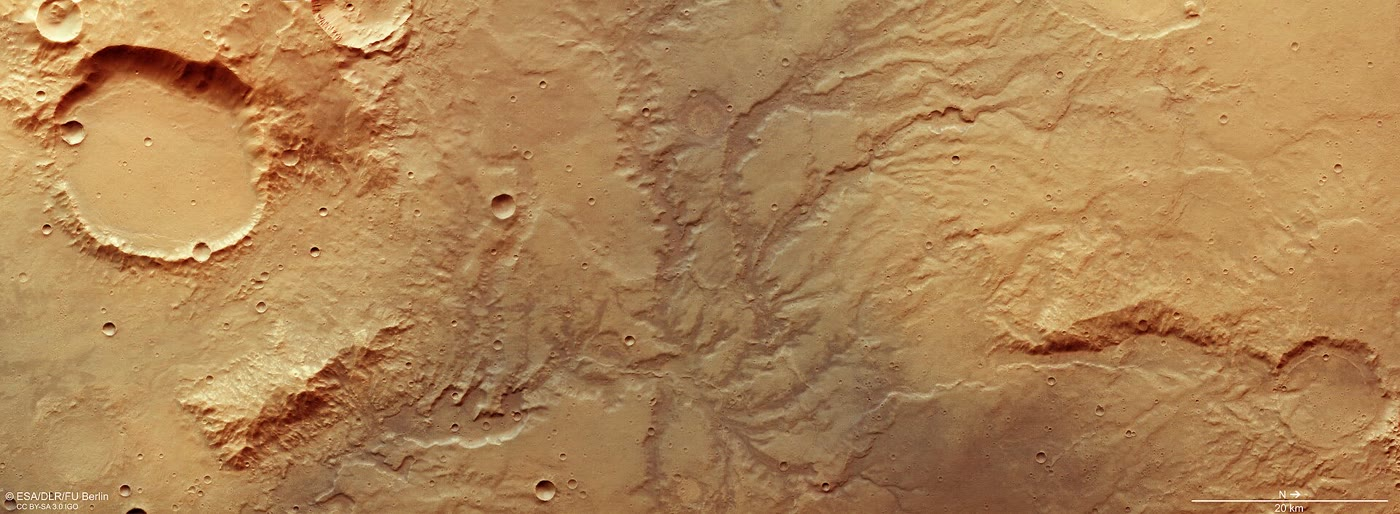
\includegraphics[width=\linewidth]{images/book5/b3-mars-valley-network.jpg}
\par\smallskip{\small شبكة من الأودية الجافّة على المريخ، كما رصدتها
كاميرا مارس إكسبريس بدقّة نحو \qty{14}{m} لكلّ بكسل، قرب \ang{17}\,جنوبًا،
\ang{66}\,شرقًا؛ والشمال نحو اليمين، وشريط المقياس يساوي \qty{20}{km}.
تنضمّ الروافد عند مصبّها إلى أودية أكبر، وهذا نمط
شبكة تصريف. الصورة: \mbox{\textdir TLT ESA/DLR/FU Berlin, CC BY-SA 3.0 IGO}.}\label{fig:b3:planetary-atmospheres:valleys}
\end{omfigure}
% ledger: photo:b3-mars-valley-network

تحتاج الأودية وقنوات الجريان على المريخ، بحسب التقديرات الجيولوجية،
إلى طبقة مائية عالمية بعمق 100 إلى \qty{1500}{m}، مقابل 3 إلى
\qty{25}{m} في جليده وهوائه اليوم. وذهب معظم الباقي إلى الفضاء. ورصدت
المركبة المدارية MAVEN أنّ الرياح الشمسية تجرّد الغاز من المريخ بمعدّل نحو
\qty{100}{g} في الثانية، ثلاثة أرباعه عبر الذيل
خلف الكوكب حيث تجري الرياح الشمسية، وربعه في العمود
فوق القطبين؛ وخلال
العواصف الشمسية في آذار 2015 تسارع الفقد، وربما كان أسرع بكثير
حين كانت الشمس الفتية أنشط. ويفقد المريخ أيضًا الهيدروجين، بنحو
\num{3e26} ذرّة في الثانية في المتوسّط اليوم، ولو استمرّ ذلك أربعة مليارات
سنة لكان الفقد يعادل طبقة مائية عالمية بعمق نحو \qty{4}{m} فقط.
% ledger: gilli25:h-loss, lasp:maven

لم يكن المعدّل دائمًا كما هو اليوم. والميل المحوري للمريخ، \ang{25.2} الآن،
تراوح بين 0 و\ang{66} خلال آخر 250 مليون سنة، حول متوسّط قرب \ang{35}،
في حين يتغيّر ميل الأرض بما لا يزيد كثيرًا على درجة واحدة.
والحركة فوضوية، ولا يمكن تتبّعها إلى الوراء عبر مليارات
السنين؛ فالفوهات الإهليلجية الناتجة عن الاصطدامات الماسّة، وتسجّل اتجاهاتها
الميل المحوري، تشير إلى متوسّط بين نحو 10 و\ang{30} خلال
آخر 3.5 مليار سنة تقريبًا. وعند الميل المحوري المرتفع يسخن القطب الصيفي،
فيرتفع مزيد من بخار الماء، وتجعل نماذج المناخ فقد الهيدروجين
أسرع بعشرين ضعفًا؛ وعبر تاريخ المريخ يعادل الفقد طبقة مائية بحدود
\qty{80}{m}.
% ledger: planet:Mars.obliq, gilli25:obliquity, holo18:obliquity, gilli25:h-loss

\section{تيتان: دورة الميثان}\label{sec:b3:planetary-atmospheres:titan}

تيتان، قمر أصغر من المريخ، يملك غلافًا جويًّا أكثف من غلاف الأرض:
ضغط سطحه أعلى بنحو 60\,\%، عند \qty{-179}{\degreeCelsius}.
ويتألّف الغلاف الجوي من نحو 95\,\% نيتروجينًا و5\,\% ميثانًا، ولأنّ
جاذبيّة القمر ضعيفة، فيمتدّ الغلاف إلى ارتفاع أعلى بعشرة أضعاف من ارتفاع غلاف الأرض،
حتى قرابة \qty{600}{km}. تفكّك الأشعّة فوق البنفسجية الميثان والنيتروجين
في الأعالي؛ وتتّحد الشظايا من جديد في ضباب برتقالي من
الهيدروكربونات الأثقل التي تحجب السطح عن الضوء المرئي. وتحت الطبقة الضبابية،
يؤدّي الميثان دور الماء: يتكثّف في سحب، ويمطر، ويحفر
قنوات الأنهار، ويملأ البحيرات والبحار المكوّنة من الميثان والإيثان.
% ledger: nasa:titan-surface, nasa:titan-facts

\begin{omfigure}
\centering
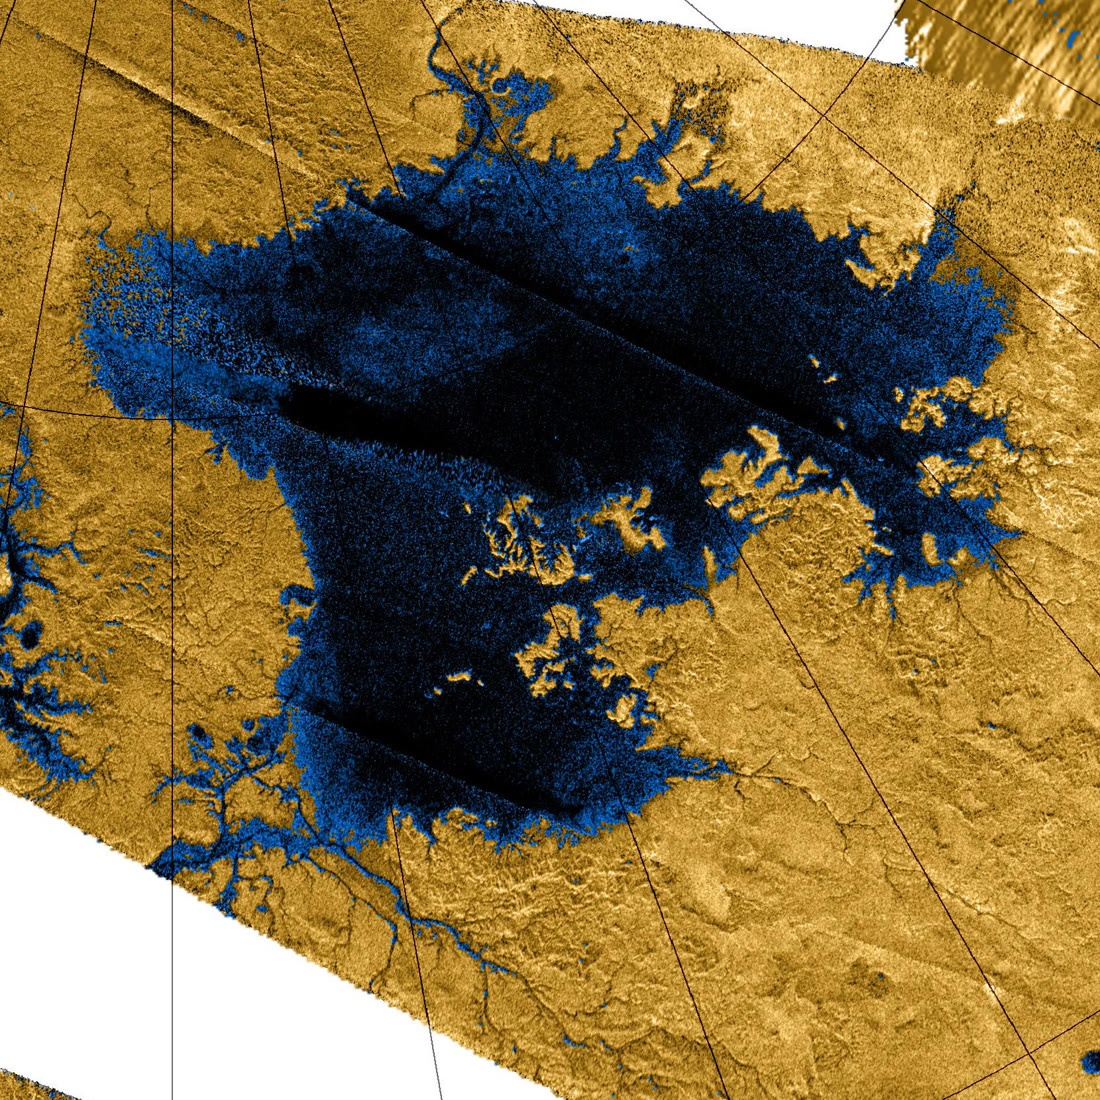
\includegraphics[width=0.5\linewidth]{images/book5/b3-ligeia-mare.jpg}
\par\smallskip{\small ليجيا ماري، بحر قرب القطب الشمالي لتيتان، في
فسيفساء بألوان كاذبة من صور رادار كاسيني: معالم يُظنّ أنّها
سائلة تظهر باللون الأزرق والأسود، وأرض صلبة مصبوغة باللون البنّي، مع خلجان وجزر
وشبكات مفترضة من الروافد. ومن نحو 400 بحيرة وبحر في المنطقة المرسومة
الشمالية، وتحوي التي تتجاوز \qty{26000}{km^2} منها 70\,\% من المساحة.
NASA/JPL/USGS، ملك عام.}\label{fig:b3:planetary-atmospheres:ligeia}
\end{omfigure}
% ledger: photo:b3-ligeia-mare

يتوقّف إمكان وجود سائل على سطح ما على مخطّط طوره،
وعلى الضغط ودرجة الحرارة عنده. ويقع سطح تيتان مباشرة فوق
النقطة الثلاثية للميثان، \qty{90.67}{K} و\qty{0.117}{bar}، وتحت
نقطته الحرجة: الميثان السائل ممكن، والميثان عند 5\,\% من
\qty{1.6}{bar} ليس بعيدًا عن التشبّع. ويقع سطح المريخ قرب
النقطة الثلاثية للماء، وسطح الأرض بعيد داخل منطقة سائل الماء، أمّا سطح الزهرة فيقع
فوق درجة الحرارة الحرجة للماء، \qty{647}{K}، حيث لا يمكن
لأيّ سائل أن يوجد أصلًا.
% ledger: nist:methane-phase, iapws:triple-critical, nasa:titan-surface

\begin{omfigure}
\centering
\begin{tikzpicture}
\begin{axis}[width=0.8\linewidth, height=0.52\linewidth,
  xmin=60, xmax=800, ymin=1e-4, ymax=1000, ymode=log,
  xlabel={درجة الحرارة \babelsublr{(\unit{K})}}, ylabel={الضغط \babelsublr{(\unit{bar})}},
  tick label style={font=\scriptsize}, label style={font=\small}]
\addplot[thick, omDef] table[x=T, y=p_bar] {figdata/out/bachelor-3-habitability-water.dat};
\addplot[thick, omDef, dashed] table[x=T, y=p_bar] {figdata/out/bachelor-3-habitability-ice.dat};
\addplot[thick, orange!80!black] table[x=T, y=p_bar] {figdata/out/bachelor-3-habitability-methane.dat};
\addplot[only marks, mark=*, mark size=1.6pt, omDef] coordinates {(273.16,0.00611657) (647.096,220.64)};
\addplot[only marks, mark=*, mark size=1.6pt, orange!80!black] coordinates {(90.67,0.1169) (190.6,46.1)};
\addplot[only marks, mark=square*, mark size=2.2pt, black] table[x=T, y=p_bar] {figdata/out/bachelor-3-habitability-bodies.dat};
\node[font=\scriptsize, anchor=south] at (axis cs:737,110) {الزهرة};
\node[font=\scriptsize, anchor=west] at (axis cs:300,1.0) {الأرض};
\node[font=\scriptsize, anchor=north] at (axis cs:214,0.0045) {المريخ};
\node[font=\scriptsize, anchor=south] at (axis cs:94,2.2) {تيتان};
\node[font=\scriptsize, omDef, anchor=west] at (axis cs:420,3) {الماء: سائل فوق وبخار تحت};
\node[font=\scriptsize, omDef, anchor=north west] at (axis cs:205,0.0012) {الجليد};
\node[font=\scriptsize, orange!80!black, anchor=west] at (axis cs:196,46) {الميثان};
\node[font=\scriptsize, omDef, anchor=south east] at (axis cs:640,230) {النقطة الحرجة};
\end{axis}
\end{tikzpicture}
\par\smallskip{\small الحدود بين البخار والماء المتكثّف
(الأزرق: سائل--بخار، من النقطة الثلاثية إلى النقطة الحرجة؛
المتقطّع: جليد--بخار)، وبين الميثان السائل وبخاره (البرتقالي)،
مع متوسّط حالات السطح للزهرة والأرض والمريخ وتيتان
(المربّعات). يمكن لسائل أن يوجد على سطح يكون ضغطه أعلى من
منحنى ذلك السائل، بين درجتي حرارته الثلاثية
والحرجة.}\label{fig:b3:planetary-atmospheres:phases}
\end{omfigure}
% ledger: iapws:vapour-pressure, iapws4:sublimation, iapws:triple-critical, nist:methane-phase, nasa:venus-atm, planet:Earth.Tmean, planet:Earth.psurf, nasa:mars-atm, nasa:titan-surface

يحتفظ تيتان بنيتروجينه بسهولة: عند قاعدة غلافه الخارجي $\lambda = 41$ من أجل
النيتروجين. أمّا هيدروجينه، عند $\lambda$ قرب 1.5، فيفلت تقريبًا بحرّية.
ويتحدّد إفلات الهيدروجين الجزيئي أدنى منه بالدفق المحدّد
عبر \omterm{def:b3:planetary-atmospheres:hydrodynamic}{حدّ التجانس}، كما على الأرض. وتستقرّ المركّبات الثقيلة المتكوّنة من
الميثان المتكسّر إلى السطح، حيث تكوّن رمال
حقول واسعة من الكثبان.
% ledger: gronoff:jeans-table, gronoff:diffusion, nasa:titan-surface

\section{صلاحية الكواكب للحياة}\label{sec:b3:planetary-atmospheres:habitability}

النطاق الصالح للحياة في كتب المدرسة هو مدى المسافات من
نجم يستطيع عنده كوكب شبيه بالأرض أن يحتفظ بالماء السائل على
سطحه. وحدّاه هما الحدّان اللذان مرّ ذكرهما في هذا الفصل.

\begin{definition}[صلاحية الكواكب للحياة]\label{def:b3:planetary-atmospheres:habitability}
\emph{صلاحية الكواكب للحياة}\index{صلاحية الكواكب للحياة} لكوكب ما
هي قدرته على الاحتفاظ بالماء السائل على سطحه عبر
الأزمنة الجيولوجية: إذ يتلقّى دفقًا نجميًّا ضمن حدود
النطاق الصالح للحياة، ويحتفظ بغلافه الجوي وبمائه ضدّ
الإفلات، ويضبط دورة الكربون طويلة الأمد مناخه.
\end{definition}

الحدّ الداخلي للنطاق الصالح للحياة هو \omterm{def:b3:planetary-atmospheres:runaway}{الدفيئة الرطبة} أو \omterm{def:b3:planetary-atmospheres:runaway}{الدفيئة
الجامحة}: كوكب شبيه بالأرض حول الشمس يتحوّل إلى دفيئة رطبة عند
\qty{0.99}{au}، وتدخل \omterm{def:b3:planetary-atmospheres:runaway}{الدفيئة الجامحة} عند \qty{0.97}{au}. أمّا الحدّ الخارجي فهو
\emph{الدفيئة القصوى}: إضافة ثاني أكسيد الكربون تدفئ الكوكب فقط حتى
يعيد الغاز الإضافي تشتيت ضوء شمسي أكثر مما يكسبه تأثيره
الدفيئي؛ ويحدث ذلك حول الشمس عند
\qty{1.70}{au}، تحت ضغط نحو \qty{8}{bar} من ثاني أكسيد الكربون. وهذه
حدود متحفّظة تُحسب بلا سحب. والحدّان التجريبيّان أوسع:
يبدو أنّ الزهرة لم تملك ماءً سطحيًّا لمدّة لا تقلّ عن مليار سنة،
حين تلقّت 1.76 مرّة ضوء الشمس الحالي الذي تتلقّاه الأرض، على بُعد \qty{0.75}{au}؛
كان للمريخ ماء جارٍ حين تلقّى 0.32 من ذلك الضوء، إذا كانت
أوديته تعود إلى 3.8 مليار سنة، على بُعد \qty{1.77}{au}. وحول النجوم الأبرد تأتي الحدود نفسها
عند دفوق أدنى، لأنّ ضوءها الأحمر يتشتّت أقلّ ويمتصّه الماء وثاني أكسيد
الكربون أكثر.
% ledger: kopparapu13:runaway, kopparapu13:outer, kopparapu13:hz-fit

\begin{omfigure}
\centering
\begin{tikzpicture}
\begin{axis}[width=0.8\linewidth, height=0.5\linewidth,
  xmin=0, xmax=2.1, ymin=2600, ymax=7200, x dir=reverse,
  xlabel={التدفّق النجمي المستلَم / تدفّق الأرض اليوم},
  ylabel={درجة حرارة النجم \babelsublr{(\unit{K})}},
  tick label style={font=\scriptsize}, label style={font=\small},
  legend style={font=\scriptsize, at={(0.5,-0.24)}, anchor=north, legend columns=2, draw=none}]
\addplot[name path=mg, thick, omDef] table[x=mg, y=Teff] {figdata/out/bachelor-3-habitability-hz.dat};
\addlegendentry{الدفيئة الرطبة}
\addplot[name path=maxg, thick, red!70!black] table[x=maxg, y=Teff] {figdata/out/bachelor-3-habitability-hz.dat};
\addlegendentry{الدفيئة القصوى}
\addplot[thin, omDef, dashed] table[x=rg, y=Teff] {figdata/out/bachelor-3-habitability-hz.dat};
\addlegendentry{الدفيئة الجامحة}
\addplot[thin, black!60, densely dotted] table[x=rv, y=Teff] {figdata/out/bachelor-3-habitability-hz.dat};
\addlegendentry{الزهرة الحديثة، المريخ المبكّر}
\addplot[thin, black!60, densely dotted, forget plot] table[x=em, y=Teff] {figdata/out/bachelor-3-habitability-hz.dat};
\addplot[green!30, opacity=0.5, forget plot] fill between[of=mg and maxg];
\addplot[only marks, mark=*, mark size=2pt, black, forget plot] coordinates {(1.911,5780) (1.0,5780) (0.431,5780)};
\node[font=\scriptsize, anchor=south] at (axis cs:1.911,5800) {الزهرة};
\node[font=\scriptsize, anchor=west, xshift=2pt] at (axis cs:1.0,5780) {الأرض};
\node[font=\scriptsize, anchor=east, xshift=-2pt] at (axis cs:0.431,5780) {المريخ};
\end{axis}
\end{tikzpicture}
\par\smallskip{\small النطاق الصالح للحياة لكوكب شبيه بالأرض، بوصفه التدفّق النجمي الذي يستلمه
مقابل درجة حرارة نجمه (مظلَّل: بين
\omterm{def:b3:planetary-atmospheres:runaway}{الدفيئة الرطبة} والدفيئة القصوى). منقّط: الحدود التجريبية
المستخلصة من الزهرة الحديثة والمريخ المبكّر. والتوفيقات هي
لنموذج مناخي خالٍ من السحب، صالح من 2600 إلى
\qty{7200}{K}.}\label{fig:b3:planetary-atmospheres:hz}
\end{omfigure}
% ledger: kopparapu13:hz-fit, nasa:venus, nasa:mars

المسافة وحدها لا تكفي. ينبغي للكوكب أن يحتفظ بغلافه الجوي: فالكوكب الصغير
أو الحارّ، الذي يكون معامل إفلاته منخفضًا، يفقد هيدروجينه ومعه
مياهه، والكوكب الواقع في دفيئة رطبة يجفّ من الأعلى. وينبغي له أيضًا أن
يحافظ على مناخه مستقرًّا عبر مليارات السنين بينما يسطع نجمه:
فعلى الأرض، يعمل منظِّم الحرارة القائم على تجوية السيليكات ضمن الدورة الكربونية طويلة الأمد
على سحب ثاني أكسيد الكربون حين يسخن المناخ، ويتركه يتراكم حين يبرد.
أمّا على الزهرة، ومن دون تكتونية صفيحية، فإنّ ثاني أكسيد الكربون المنبعث
لم يجد سبيلًا للعودة إلى الصخور، فتراكم في الجو؛ وهو يحتوي اليوم على قدر
يقارب ما حبسته الأرض في الصخور الكربوناتية من ثاني أكسيد الكربون.
ولا يزال الجدل قائمًا حول ما إذا كان المجال المغناطيسي يحمي
الغلاف الجوي: فهو يحجب الغلاف العلوي عن الرياح الشمسية، لكنّه يفتح
كذلك مسارات إفلات أخرى، مثل خروج الأيونات
قرب القطبين، وصلاحية الكوكب للحياة لا تُقرأ من موقعه
في النطاق الصالح للحياة وحده.
% ledger: arney18:venus-loss, gronoff21:magnetic, gronoff:nonthermal

\section{التمارين}

\begin{exercise}[$\star$]\label{exo:b3:planetary-atmospheres:1}
احسب ارتفاع المقياس $H = RT/Mg$ قرب سطح الزهرة
(عند \qty{737}{K}، وثاني أكسيد الكربون بكتلة مولية \qty{44.01}{g.mol^{-1}}،
$g = \qty{8.87}{m.s^{-2}}$)، والأرض (عند \qty{288}{K}،
\qty{28.97}{g.mol^{-1}}، \qty{9.80}{m.s^{-2}})، والمريخ (عند \qty{214}{K}،
\qty{43.34}{g.mol^{-1}}، \qty{3.71}{m.s^{-2}})، وتيتان (عند \qty{94}{K}،
\qty{28.0}{g.mol^{-1}}، \qty{1.35}{m.s^{-2}}). أيّ الأغلفة الجوية هو الأكثر
امتدادًا، ولماذا؟
\end{exercise}

\begin{exercise}[$\star$]\label{exo:b3:planetary-atmospheres:2}
تقع \omterm{def:b3:planetary-atmospheres:exobase}{قاعدة الغلاف الخارجي} للأرض عند \qty{500}{km} (نصف القطر \qty{6878}{km})؛ وتتغيّر
درجة حرارتها من 800 إلى \qty{1600}{K} على امتداد الدورة الشمسية. ونأخذ
كتلة الأرض \qty{5.97e24}{kg}. احسب \omterm{def:b3:planetary-atmospheres:jeans-escape}{معامل الإفلات} لذرات الهيدروجين عند الحرارتين،
وكسر الذرات المنفلتة،
$(1 + \lambda)e^{-\lambda}$. وبأيّ عامل تغيّره الدورة الشمسية؟
\end{exercise}

\begin{exercise}[$\star$]\label{exo:b3:planetary-atmospheres:3}
حول الشمس، يتحوّل كوكب شبيه بالأرض إلى دفيئة رطبة عند التدفّق $S_\mathrm{eff}
= 1.014$، تبلغ \omterm{def:b3:planetary-atmospheres:runaway}{الدفيئة الجامحة} عند 1.0512، وتبلغ الدفيئة القصوى عند 0.3438
(التدفّقات نسبةً إلى تدفّق الأرض). (أ)~احسب المسافات الثلاث بالوحدات
الفلكية. (ب)~تتلقّى الزهرة والمريخ 1.91 و0.43 مرّة من ضوء الشمس الذي تتلقّاه الأرض.
حدّد موضعيهما.
\end{exercise}

\begin{exercise}[$\star$]\label{exo:b3:planetary-atmospheres:4}
يُعطى ضغط بخار الميثان السائل بالعلاقة $\log_{10}(p/\unit{bar}) = 3.9895 -
443.028/(T/\unit{K} - 0.49)$. (أ)~احسب هذا الضغط عند سطح تيتان،
\qty{94.15}{K}. (ب)~يشكّل الميثان 5\,\% من هواء تيتان عند \qty{1.6}{bar}.
احسب ضغطه الجزيئي ورطوبته النسبية. (ج)~ما الذي توحي به النتيجة
بشأن التبخّر من بحار تيتان؟
\end{exercise}

\begin{exercise}[$\star\star$]\label{exo:b3:planetary-atmospheres:5}
عند \omterm{def:b3:planetary-atmospheres:exobase}{قاعدة الغلاف الخارجي} للأرض (عند \qty{1000}{K}، و$\lambda = 7.02$ للهيدروجين)،
احسب \omterm{def:b3:planetary-atmospheres:jeans-escape}{معامل الإفلات} للديوتيريوم، وسرعته الحرارية نسبةً إلى سرعة الهيدروجين،
ونسبة دفقي \omterm{def:b3:planetary-atmospheres:jeans-escape}{إفلات جينز} لكلّ ذرّة، من D إلى H. هل يُعدّ \omterm{def:b3:planetary-atmospheres:jeans-escape}{إفلات جينز}
مرشّحًا نظيريًّا قويًّا؟
\end{exercise}

\begin{exercise}[$\star\star$]\label{exo:b3:planetary-atmospheres:6}
نسبة D/H في مياه الزهرة \num{0.016}؛ أمّا في مياه محيطات الأرض فهي
\num{1.5575e-4}. (أ)~احسب مقدار الإثراء. (ب)~بافتراض ألّا يفلت الديوتيريوم البتّة، ما أصغر
مخزون ماضٍ من مياه الزهرة ممكن، علمًا بأنّ مخزونها اليوم \qty{6e15}{kg}؟ وما العمق الذي
يبلغه هذا المخزون لو توزّع على سطح الكوكب البالغ مساحته \qty{4.60e14}{m^2}؟ (ج)~أيّ
تقلّص في الخزّان يتطلّبه \omterm{def:b3:planetary-atmospheres:hydrodynamic}{الإفلات المحدود بالانتشار}، إذا كان $\alpha = 0.8$؟
استنتج.
\end{exercise}

\begin{exercise}[$\star\star$]\label{exo:b3:planetary-atmospheres:7}
يفقد المريخ، ونصف قطره \qty{3389.5}{km}، نحو \num{3e26} ذرّة هيدروجين
في الثانية. (أ)~إذا كان كلّ زوج من الذرات قد نشأ عن جزيء ماء، فما الطبقة
المائية الشاملة التي يزيلها هذا الفقد خلال أربعة مليارات سنة؟
(ب)~السؤال نفسه عند \num{6e27} ذرّة في الثانية، وهو معدّل الميل المحوري
المرتفع. (ج)~قارن ذلك بالمدى من 100 إلى \qty{1500}{m} الذي تحتاجه الأودية
والقنوات.
\end{exercise}

\begin{exercise}[$\star\star$]\label{exo:b3:planetary-atmospheres:8}
(أ)~احسب كتلة الغلاف الجوي للمريخ انطلاقًا من متوسط
الضغط السطحي \qty{636}{Pa}، وجاذبيته \qty{3.71}{m.s^{-2}}،
ونصف قطره. (ب)~تنزع الرياح الشمسية نحو \qty{100}{g} من الغاز في الثانية.
ما الكتلة التي يزيلها ذلك خلال أربعة مليارات سنة، وخلال كم من الزمن
سيزيل الغلاف الجوي الحالي؟ (ج)~لماذا يُعدّ ذلك تقديرًا ناقصًا للفقد
في الماضي؟
\end{exercise}

\begin{exercise}[$\star\star$]\label{exo:b3:planetary-atmospheres:9}
يعكس كوكب شبيه بالأرض، يملك غلافًا جويًا من البخار الخالي من السحب، 19.3\,\%
من ضوء الشمس الذي يتلقّاه؛ ولا يمكن أن يتجاوز إشعاعه تحت الأحمر
\qty{291}{W.m^{-2}}. (أ)~فوق أيّ تدفّق للضوء الشمسي، بالواط في كلّ متر
مربّع، ونسبةً إلى ثابت الشمس للأرض \qty{1361}{W.m^{-2}}، يدخل الكوكب في \omterm{def:b3:planetary-atmospheres:runaway}{الدفيئة الجامحة}؟
(ب)~قارن بالزهرة اليوم، \qty{2601}{W.m^{-2}}، وبالزهرة الفتيّة
تحت شمس بإشعاعية 70\,\% من إشعاعيتها الحالية. (ج)~لماذا لا يكون
الاستنتاج الخاص بالزهرة الفتيّة نهائيًا؟
\end{exercise}

\begin{exercise}[$\star\star\star$]\label{exo:b3:planetary-atmospheres:10}
غلاف حراري نموذجي من الأكسجين الذرّي متساوي الحرارة عند \qty{1000}{K}، مع
$n = \qty{1e16}{m^{-3}}$ عند \qty{200}{km}؛ خذ $g =
\qty{9.21}{m.s^{-2}}$ عند ذلك الارتفاع، ومقطع التصادم العرضي
$\sigma_c = \qty{3e-19}{m^2}$. (أ)~احسب ارتفاع المقياس للأكسجين.
(ب)~احسب الكثافة عند \omterm{def:b3:planetary-atmospheres:exobase}{قاعدة الغلاف الخارجي} وارتفاع \omterm{def:b3:planetary-atmospheres:exobase}{قاعدة الغلاف الخارجي}.
(ج)~تتناقص الجاذبية مع الارتفاع. هل يرفع ذلك \omterm{def:b3:planetary-atmospheres:exobase}{قاعدة الغلاف الخارجي} أم
يخفضها؟
\end{exercise}

\begin{exercise}[$\star\star\star$]\label{exo:b3:planetary-atmospheres:11}
(أ)~لنفترض أنّ الستراتوسفير على الأرض أصبح رطبًا، بنسبة خلط لبخار الماء
\num{3e-3} (محسوبةً بوصفها $\ce{H2}$). ومع
حدّ الانتشار $\num{3.0e13}\,f$ جزيئًا من $\ce{H2}$ لكلّ سنتيمتر مربّع
وفي الثانية، عند \qty{200}{K}، احسب فقد الهيدروجين لكامل الأرض
(نصف قطرها \qty{6371}{km}). (ب)~كم تدوم مياه محيط يبلغ مقدارها
\qty{1.4e24}{g} من الماء؟ قارن ذلك بعمر الأرض.
\end{exercise}

\begin{exercise}[$\star\star\star$]\label{exo:b3:planetary-atmospheres:12}
في غلاف جوي علوي من البخار النقي يمتصّ كغاز رمادي، بمعامل امتصاص $\kappa =
\qty{0.005}{m^2.kg^{-1}}$، على كوكب جاذبيته $g = \qty{9.81}{m.s^{-2}}$
و$D = 1.66$: (أ)~احسب الضغط $p_1$ عند مستوى الإشعاع؛
(ب)~باستخدام $p_\mathrm{sat}(T) = \qty{611.657}{Pa}\,\exp[(L/R_v)(1/T_t -
1/T)]$, $L = \qty{2.5e6}{J.kg^{-1}}$, $R_v = \qty{461.5}{J.kg^{-1}.K^{-1}}$,
$T_t = \qty{273.16}{K}$، احسب درجة حرارته وحدّ الإشعاع.
(ج)~حدّ الحساب سطرًا بسطر هو \qty{291}{W.m^{-2}}. هل ينبغي أن يكون المعامل
$\kappa$ الفعّال لبخار الماء الحقيقي أكبر أم أصغر؟
\end{exercise}

\section{مسألة: هل يحتفظ كيبوس بمائه؟}

\begin{problem}[{مسألة نهاية الأسبوع --- الإفلات وصلاحية الكواكب للحياة في كوكب
محيطيّ مُتخيَّل}]
\label{pb:b3:planetary-atmospheres:1}
كيبوس كوكب مُتخيَّل كتلته \qty{5.2e24}{kg} ونصف قطره
\qty{6200}{km}، وله محيطات وغلاف جوي من النيتروجين وثاني
أكسيد الكربون. يدور على بعد \qty{0.60}{au} من نجم إشعاعيته 0.30 مرّة من إشعاعية
الشمس، ودرجة حرارته الفعّالة \qty{4800}{K}. تقع قاعدة غلافه الخارجي
على ارتفاع \qty{500}{km} فوق السطح، عند \qty{1400}{K}، مع
\qty{2e11}{m^{-3}} من ذرّات الهيدروجين؛ ويقع حدّ تجانسه عند \qty{200}{K}،
حيث يهيمن ثاني أكسيد الكربون، وحيث يشكّل الهيدروجين بكلّ صوره
نسبة الخلط $f = \num{1e-3}$، محسوبةً بوصفها $\ce{H2}$. ومحيط الأرض يساوي
\qty{1.4e24}{g} من الماء.

\medskip\noindent\textbf{الجزء الأول --- \omterm{def:b3:planetary-atmospheres:exobase}{قاعدة الغلاف الخارجي}.}
\begin{enumerate}
\item احسب جاذبية السطح ومتوسط كثافة كيبوس.
\item احسب سرعة الإفلات عند \omterm{def:b3:planetary-atmospheres:exobase}{قاعدة الغلاف الخارجي}.
\item احسب السرعة الحرارية $u = \sqrt{2kT/m}$ لذرّات الهيدروجين والهيليوم
  والأكسجين عند \omterm{def:b3:planetary-atmospheres:exobase}{قاعدة الغلاف الخارجي}.
\item احسب معاملات الإفلات لكلّ منها.
\item أيّ منها يمكنه الإفلات بمعدّل ملحوظ وفق \omterm{def:b3:planetary-atmospheres:jeans-escape}{إفلات جينز}؟
  هل يقترب أيّ منها من نظام \omterm{def:b3:planetary-atmospheres:hydrodynamic}{الإفلات الهيدروديناميكي}؟
\item خلال مرحلة الشباب النشط لنجمه ربما وصلت \omterm{def:b3:planetary-atmospheres:exobase}{قاعدة الغلاف الخارجي} لكيبوس
  إلى \qty{3000}{K}. فما معامل إفلات الهيدروجين آنذاك،
  وماذا يوحي ذلك؟
\end{enumerate}

\medskip\noindent\textbf{الجزء الثاني --- \omterm{def:b3:planetary-atmospheres:jeans-escape}{إفلات جينز} للهيدروجين.}
\begin{enumerate}[resume]
\item احسب الكسر المنفلت $(1 + \lambda)e^{-\lambda}$ لذرّات
  الهيدروجين.
\item احسب دفق جينز للهيدروجين، في كلّ متر مربّع وفي الثانية.
\item احسب عدد ذرّات الهيدروجين التي تغادر كامل \omterm{def:b3:planetary-atmospheres:exobase}{قاعدة الغلاف الخارجي}
  في الثانية.
\item كم عدد ذرّات الهيدروجين التي يحتوي عليها محيط الأرض؟
\item بهذا المعدّل، كم يستغرق كيبوس لفقدها؟
\item احسب معامل إفلات الديوتيريوم وكفاءة إفلاته
  بالنسبة إلى الهيدروجين، لكلّ ذرّة.
\end{enumerate}

\medskip\noindent\textbf{الجزء الثالث --- حدّ الانتشار.}
\begin{enumerate}[resume]
\item احسب ارتفاع المقياس لثاني أكسيد الكربون عند \omterm{def:b3:planetary-atmospheres:hydrodynamic}{حدّ التجانس}.
\item معامل الانتشار الثنائي للهيدروجين في ثاني أكسيد الكربون هو
  $b = \qty{1.2e19}{cm^{-1}.s^{-1}}$ عند \qty{200}{K}. احسب
  دفق \omterm{def:b3:planetary-atmospheres:hydrodynamic}{الإفلات المحدود بالانتشار} لجزيئات $\ce{H2}$، في كلّ متر مربّع وفي الثانية.
\item تحقّق من ذلك مقارنةً بحدّ الأرض، $\num{3.0e13}\,f$ جزيئًا في
  كلّ سنتيمتر مربّع وفي الثانية، مُعدَّلًا بالجاذبية.
\item احسب عدد ذرّات الهيدروجين التي يمكن أن يزوّد بها حدّ الانتشار
  الغلاف الجوي العلوي للكوكب بأكمله في الثانية (خذ
  مساحة السطح).
\item قارن بالسؤال~9. أيّ عملية تحدّ من الإفلات، وماذا
  يحدث لهيدروجين الغلاف الحراري؟
\item ما كثافة الهيدروجين عند \omterm{def:b3:planetary-atmospheres:exobase}{قاعدة الغلاف الخارجي} التي تجعل \omterm{def:b3:planetary-atmospheres:jeans-escape}{إفلات جينز} يحمل
  الإمداد كلّه؟
\item كم يستغرق كيبوس لفقد محيط الأرض من الهيدروجين عند
  \omterm{def:b3:planetary-atmospheres:hydrodynamic}{الإفلات المحدود بالانتشار}؟
\end{enumerate}

\medskip\noindent\textbf{الجزء الرابع --- هل يقع كيبوس في النطاق الصالح للحياة؟}
\begin{enumerate}[resume]
\item احسب الدفق النجمي الذي يتلقّاه كيبوس، نسبةً إلى ما تتلقّاه الأرض.
\item بالنسبة إلى نجم حرارته \qty{4800}{K} يقع حدّ \omterm{def:b3:planetary-atmospheres:runaway}{الدفيئة الرطبة} عند
  $S_\mathrm{eff} = 0.939$، وحدّ الدفيئة القصوى عند 0.290. احسب
  حدود النطاق الصالح للحياة بالوحدات الفلكية، وحدّد موضع كيبوس.
\item بأيّ معامل ينبغي أن يزداد سطوع النجم قبل أن يبلغ كيبوس
  الحافة الداخلية؟
\item مع ألبيدو قدره 0.3، احسب ضوء الشمس الذي يمتصّه كيبوس لكلّ متر
  مربّع، ودرجة حرارة التوازن لها. قارن \omterm{def:b3:planetary-atmospheres:runaway}{بحدّ الدفيئة
  الجامحة}.
\item لو جعل مناخٌ أدفأ ستراتوسفير كيبوس رطبًا، مع
  $f = \num{3e-3}$، كم تدوم مياه محيط الأرض؟
\item أعطِ الزمن الذي يفقد فيه كيبوس محيط الأرض من الهيدروجين \omterm{def:b3:planetary-atmospheres:hydrodynamic}{بالإفلات
  المحدود بالانتشار} عند $f = \num{1e-3}$، بمليارات السنين، إلى
  رقمين معنويّين.
\end{enumerate}
\end{problem}
% ledger: zahnle19:diffusion, kopparapu13:hz-fit, kopparapu13:runaway, gronoff:jeans, const:G, const:kB, const:NA
